% Copyright 2004 by Till Tantau <tantau@users.sourceforge.net>.
%
% In principle, this file can be redistributed and/or modified under
% the terms of the GNU Public License, version 2.
%
% However, this file is supposed to be a template to be modified
% for your own needs. For this reason, if you use this file as a
% template and not specifically distribute it as part of a another
% package/program, I grant the extra permission to freely copy and
% modify this file as you see fit and even to delete this copyright
% notice. 

\documentclass{beamer}
%\documentclass{beamer}
\usepackage{blindtext}
\usepackage{graphicx}
\usepackage{multirow}
\usepackage{multicol}
\usepackage{booktabs}
\usepackage{adjustbox}
\usepackage{subfiles}
\usepackage{amsmath}
\usepackage{amsthm}
\usepackage{tikz}
\usepackage{wrapfig}
\usepackage{lscape}
\usepackage{rotating}
\usepackage{epstopdf}
\usepackage{subcaption}
\usepackage[font=small,labelfont=bf]{caption}
\usepackage{hyperref}
\usepackage{color}
\usepackage{verbatim}
\usepackage{algorithm}% http://ctan.org/pkg/algorithms
\usepackage{algpseudocode}% http://ctan.org/pkg/algorithmicx
\usetikzlibrary{shapes.geometric, arrows}
\theoremstyle{definition}
\theoremstyle{remark}
\newtheorem*{remark}{Remark}
\usepackage{amssymb}
\usepackage{amsfonts}
\usepackage{mathtools}
\usepackage{adjustbox}
\newcommand{\defeq}{\vcentcolon=}
\newcommand{\eqdef}{=\vcentcolon}
\newcommand*{\V}[1]{\mathbf{#1}}%
\newcommand{\norm}[1]{\left\lVert#1\right\rVert}
\newcommand{\justif}[2]{&{#1}&\text{#2}}
\newcommand{\qedwhite}{\hfill \ensuremath{\Box}}
\newcommand\given[1][]{\:#1\vert\:}
\newcommand{\me}{\mathrm{e}}
\DeclarePairedDelimiterX{\infdivx}[2]{(}{)}{%
  #1\;\delimsize\|\;#2%
}
\DeclarePairedDelimiter\abs{\lvert}{\rvert}%
\newcommand{\Conv}{\mathop{\scalebox{1.5}{\raisebox{-0.2ex}{$\ast$}}}}%
\newcommand{\infdiv}{\infdivx}
\newcommand{\parder}[2]{\frac{\partial{#1}}{\partial{#2}}}
\renewcommand{\qed}{\hfill\blacksquare}
% Bibliography package and style
\usepackage[sorting=nyt,backend=bibtex,bibstyle=authoryear,natbib=true]{biblatex}
%\setlength{\bibhang}{0pt}
%\setlength{\bibsep}{m}

%\usepackage[backend=bibtex,
%style=alphabetic,
%citestyle=authoryear]{biblatex}
%\bibliography{abbati_transfer.bib}
\addbibresource{bib.bib}
% There are many different themes available for Beamer. A comprehensive
% list with examples is given here:
% http://deic.uab.es/~iblanes/beamer_gallery/index_by_theme.html
% You can uncomment the themes below if you would like to use a different
% one:
%\usetheme{AnnArbor}
%\usetheme{Antibes}
%\usetheme{Bergen}
%\usetheme{Berkeley}
%\usetheme{Berlin}
%\usetheme{Boadilla}
%\usetheme{boxes}
%\usetheme{CambridgeUS}
%\usetheme{Copenhagen}
%\usetheme{Darmstadt}
%\usetheme{default}
%\usetheme{Frankfurt}
%\usetheme{Goettingen}
%\usetheme{Hannover}
%\usetheme{Ilmenau}
%\usetheme{JuanLesPins}
%\usetheme{Luebeck}
%\usetheme{Madrid}
%\usetheme{Malmoe}
%\usetheme{Marburg}
%\usetheme{Montpellier}
%\usetheme{PaloAlto}
%\usetheme{Pittsburgh}
\usetheme{Rochester}
%\usetheme{Singapore}
%\usetheme{Szeged}
%\usetheme{Warsaw}
\newcommand{\newauthor}[2]{
  \parbox{0.26\textwidth}{
    \texorpdfstring
      {
        \centering
        #1 \\
        {\scriptsize{\urlstyle{same}\url{#2}\urlstyle{tt}}}
      }
      {#1}
  }
}



\author{
  \newauthor{Bernardo P\'erez Orozco}{ber@robots.ox.ac.uk}
\and
  \newauthor{Gabriele Abbati}{gabb@robots.ox.ac.uk}
\and
  \newauthor{Steve Roberts}{sjrob@robots.ox.ac.uk}
}

\title{MOrdRed: Memory-based Ordinal Regression Deep Neural Networks}

% A subtitle is optional and this may be deleted
%\subtitle{A succinct introduction}

%\author{Bernardo P\'erez Orozco \and Gabriele Abbati \and Steve Roberts}
% - Give the names in the same order as the appear in the paper.
% - Use the \inst{?} command only if the authors have different
%   affiliation.

\institute[University of Oxford] % (optional, but mostly needed)
{
  Machine Learning Research Group\\Department of Engineering Sciences\\
  University of Oxford}
% - Use the \inst command only if there are several affiliations.
% - Keep it simple, no one is interested in your street address.

\date{30 August 2018}
% - Either use conference name or its abbreviation.
% - Not really informative to the audience, more for people (including
%   yourself) who are reading the slides online

\subject{Machine Learning}
% This is only inserted into the PDF information catalog. Can be left
% out. 

% If you have a file called "university-logo-filename.xxx", where xxx
% is a graphic format that can be processed by latex or pdflatex,
% resp., then you can add a logo as follows:

% \pgfdeclareimage[height=0.5cm]{university-logo}{university-logo-filename}
% \logo{\pgfuseimage{university-logo}}

% Delete this, if you do not want the table of contents to pop up at
% the beginning of each subsection:
\AtBeginSubsection[]
{
  \begin{frame}<beamer>{Outline}
    \tableofcontents[currentsection,currentsubsection]
  \end{frame}
}

% Let's get started
\begin{document}

\begin{frame}
  \titlepage
\end{frame}



% Section and subsections will appear in the presentation overview
% and table of contents.


\begin{frame}{Outline}
  \tableofcontents
  % You might wish to add the option [pausesections]
\end{frame}

\setbeamercolor{normal text}{fg=gray,bg=}
\setbeamercolor{alerted text}{fg=black,bg=}
\usebeamercolor{normal text}

\section{Time Series Forecasting}
\frame{\tableofcontents[currentsection]}
\begin{frame}{Time Series Forecasting}
  \begin{itemize}
    \item \alert<+>{Time series forecasting (TSF) is ubiquitous:}
    {
        \begin{itemize}
            \item \alert<+> {Health care, Astronomy, Finance, Energy industry}
        \end{itemize} \pause
    }
    
     \item \alert<+>{TSF is more than minimising MSE:}
    {
        \begin{itemize}
            \item \alert<+> {\textbf{Reliable} accurate bounds: uncertainty in phase and magnitude}
            \item \alert<+> {\textbf{Shape} of the predictive posterior?} 
            \item \alert<+> {\textbf{End-to-end} pipeline?}
            \item \alert<+> {\textbf{Scalable} methods for big data}
        \end{itemize} \pause
    }
    
    \item \alert<+>{Dominated by statistical (\& often parametric) models:}
    {
        \begin{itemize}
            \item \alert<+> {Gaussian Processes, ARIMA}
            \item \alert<+> {Expert knowledge may be required to e.g. design a kernel}
        \end{itemize} \pause
    }
  \end{itemize}
\end{frame}

\subsection{Ordinal Regression}
\begin{frame}{Ordinal (Auto-)Regression}
    \begin{itemize}
        \item \alert<+> {Let $\mathbf{x}$ be a bounded time series with range $I$, and let $C=(C_1, \dots, C_M)$ be a coarse-grained interval partition over $I$.} 
        \item \alert<+> {\textbf{Ordinal (auto-)regression}: For a lookback frame of $P$ one-hot encoded observations $\mathbf{X}^{(t)} = (\mathbf{x}_{t-P-1}, \dots, \mathbf{x}_t), \mathbf{x}_k\in \mathbb{R}^M$, forecast $\hat{\mathbf{x}}_{t+1}\in \mathbb{R}^M$}
        \item \alert<+>{Ordinal predictive distributions over $C$ can describe rich multi-modal, non-Gaussian behaviour.}
    \end{itemize}
\end{frame} 

\begin{frame}{Bridging ordinal regression and neural networks}
    \begin{itemize}
    \item \alert<+> {Ordinal autoregression is a discrete symbol sequence learning task. }\pause
    \item \alert<+> {NLP: Long Short-Term Memory's success: }\pause
    \begin{itemize}
        \item \alert<+> {Recurrent model that can be learnt by gradient descent }
        \item \alert<+> {Scales with data and number of classes }
        \item \alert<+> {Dropout-based approximation enables principled construction of error bounds \cite{gal2016theoretically} }\pause
    \end{itemize}
    \item \alert<+>{Softmax densities have multiple interpretations:} \pause
        \begin{itemize}
            \item \alert<+>{Categorical distribution over partition $C$}
            \item \alert<+>{Stepwise uniform distribution over original time series range $I$} \pause
        \end{itemize}
    \end{itemize}
\end{frame}

\begin{frame}{Memory-based ordinal deep neural networks}
  \begin{itemize}
    \item \alert<+> {Our proposal: recast time series forecasting as ordinal regression, then use recurrent neural networks to do forecasting.}\pause
    {
        \begin{itemize}
            \item \alert<+> {Ordinal regression $\rightarrow$ \textbf{shape flexibility}}
            \item \alert<+> {Dropout as approximate Bayes \citep{pmlr-v48-gal16} $\rightarrow$ principled (though approximate) \textbf{uncertainty bounds}}
            \item \alert<+> {Recurrent neural networks $\rightarrow$ \textbf{scalability}}
            \item \alert<+> {No need to design a kernel or extract features $\rightarrow$ \textbf{end-to-end}}
        \end{itemize} \pause
    }
  \end{itemize}
\end{frame}

\subsection{Sequence-to-sequence neural nets}
\begin{frame}{Sequence-to-sequence learning}
    \begin{itemize}
        \item \alert<+>{Sequence-to-sequence \cite{Sutskever2014} jointly learns two models: a \textit{bidirectional recurrent encoder} and a \textit{recurrent decoder}.}\pause
        \item \alert<+>{The encoder maps the lookback sequence $\mathbf{X}^{(t-1)}$ into fixed-dimensional feature vectors $\mathbf{h}_0^{(\text{dec})}, \mathbf{C}_0^{(\text{dec})}$.} \pause 
        \item \alert<+>{The decoder performs the actual autoregressive forecasting, i.e.}:
        \begin{itemize}
            \item \alert<+>{$\mathbf{h}_0^{(\text{dec})}, \mathbf{C}_0^{(\text{dec})} = f^{(enc)}(\mathbf{X}^{(t-1)})$}
            \item \alert<+>{$\hat{\mathbf{y}}_t = \text{Softmax}\left(f^{(dec)}(\mathbf{h}_{t-1}, \mathbf{C}_{t-1})\right)$}
        \end{itemize}
    \end{itemize}
    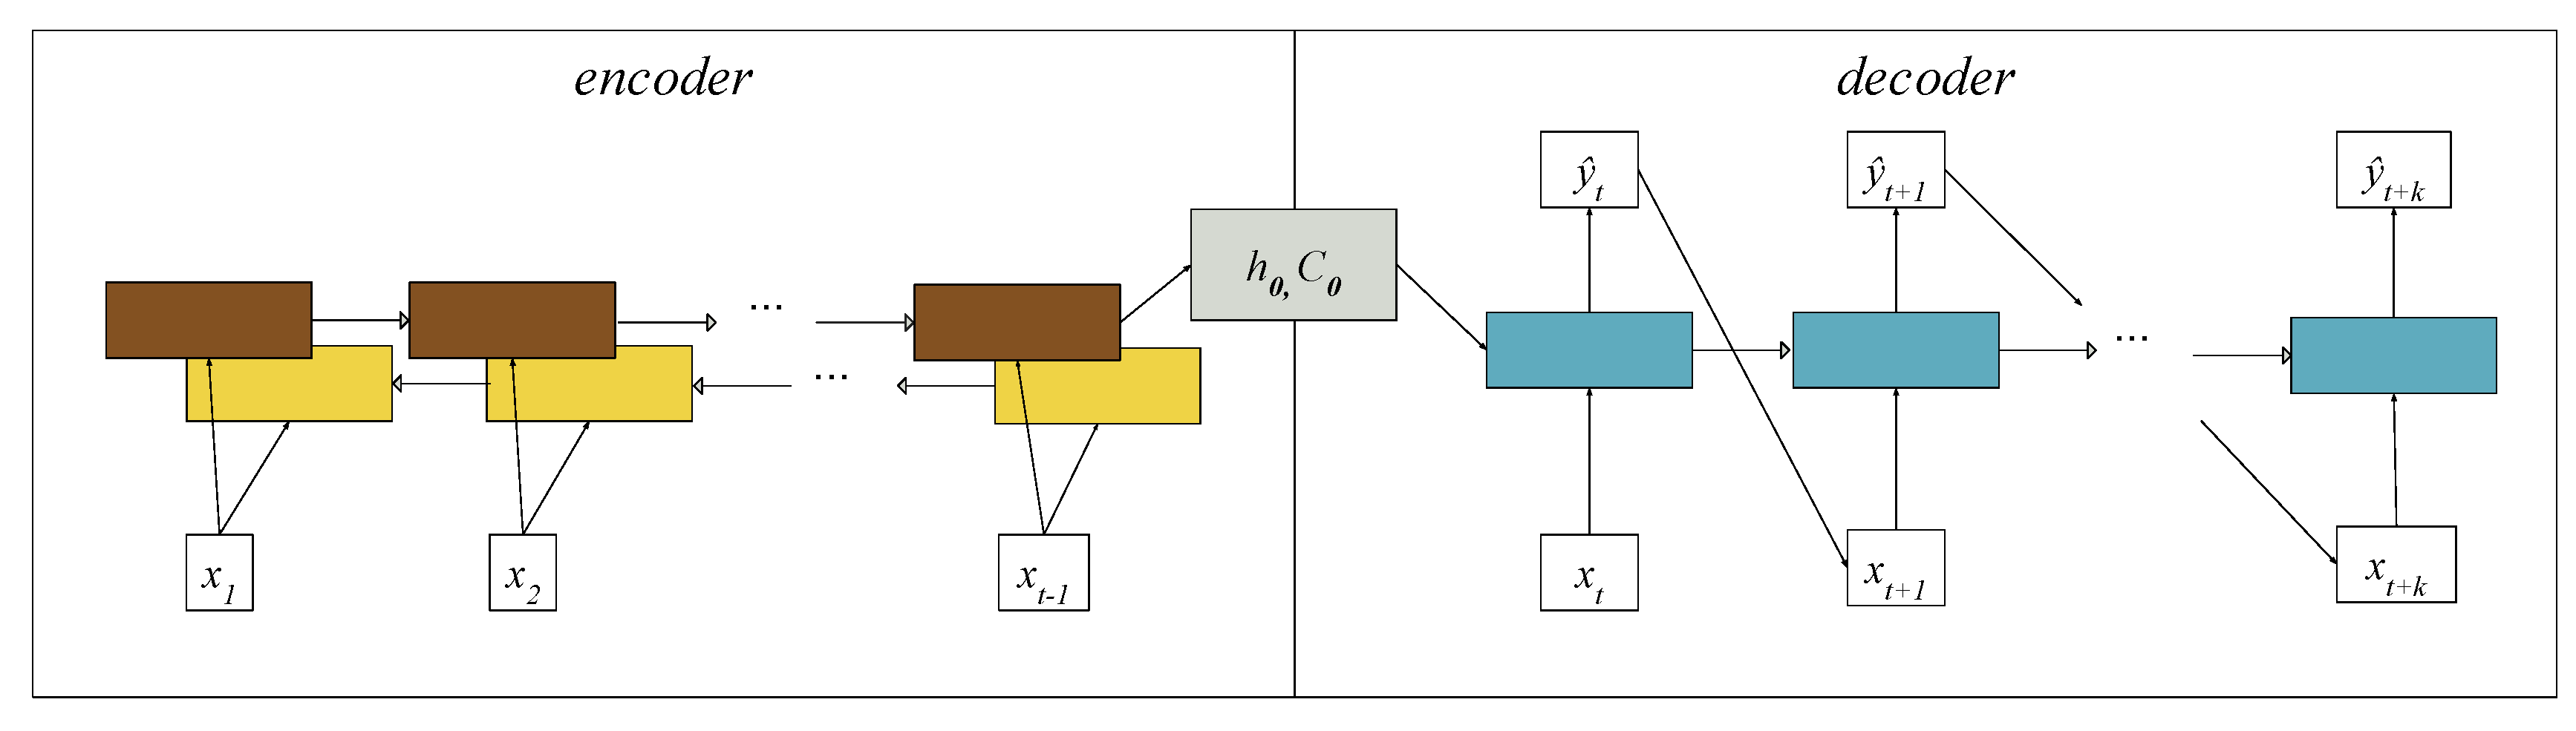
\includegraphics[width=11cm]{plots/Seq2Seq.pdf}
\end{frame}

\section{Evaluation}
\frame{\tableofcontents[currentsection]}
\subsection{Reliable long-term time series forecasting}
\begin{frame}{Evaluation: Reliable long-term forecasting}
    \begin{itemize}
        \item \alert<+>{\textbf{Goal: } Forecast $P_h$ samples from $P$-sample-long lookback frame, $P << P_h$. We choose $P=100, P_h=1000$} \pause 
        \item \alert<+>{\textbf{Baselines: }} \begin{itemize}
            \item \alert<+>{Autoregressive Gaussian Process with Gaussian emissions}
            \item \alert<+>{Autoregressive Gaussian Process with GMM emissions}
            \item \alert<+>{Trivial baseline: LSTM that performs direct regression}
            \item \alert<+>{State-space formulation of AR($p$)} \pause
        \end{itemize}    
        \item \alert<+>{\textbf{Data:}}
        \begin{itemize}
            \item \alert<+>{45 datasets drawn from a massive compilation \citep{Fulcher20130048}.} 
            \item \alert<+>{Variety of domains: meteorological, acoustic, dynamical systems etc.}
            \item \alert<+>{All time series must have at least 10,000 observations.}
        \end{itemize}
        
    \end{itemize}
\end{frame}

\begin{frame}{Evaluation: criteria and metrics}
    \begin{itemize}
        \item \alert<+>{\textbf{Uncertainty quantification:}
        \begin{itemize}
            \item Negative log likelihood, 
            \item Cumulative negative log likelihood, 
        \end{itemize}
        }
        \item \alert<+>{\textbf{Uncertainty calibration:}
        \begin{itemize}
            \item QQDist: Euclidean distance between the identity and the predictive posterior quantile-quantile curve.
            \item QQDist-250: Same as above, but only up to $P_h=250$
        \end{itemize}
        }
        \item \alert<+>{\textbf{Median forecast deviation:}
        \begin{itemize}
            \item Mean Absolute Scaled Error (MASE), 
            \item Symmetric Mean Absolute Percent Error (SMAPE).
        \end{itemize}
        }
    \end{itemize}
\end{frame}


\begin{frame}{Results}
\begin{table} \centering
\adjustbox{max height=\dimexpr\textheight-5.5cm\relax,
           max width=\textwidth}{
\begin{tabular}{lrrrrrr}
\toprule
{} &     NLL &  CumNLL &  QQ Dist &  QQ Dist 250 &  SMAPE &  MASE \\
\midrule
\textbf{MOrdReD           } & \textbf{0.8000} &          \textbf{0.7778} &   \textbf{1.1333} &       \textbf{1.1556} &         \textbf{0.8444} &        \textbf{1.0444} \\
\textbf{Best-performing GP           } & 1.4444 &          1.2000 &   1.5778 &       1.8222 &         1.4000 &        1.4444 \\
\textbf{AR(p)           } & 1.4444 &          1.7556 &   1.3333 &       1.2000 &         1.8667 &        1.5333 \\
\textbf{Seq2Seq regression} & 2.3111 &          2.2667 &   1.9556 &       1.8222 &         1.8889 &        1.9778 \\
\bottomrule
\end{tabular}
}
\caption{Average performance rank achieved by each model for each metric, where rank 0 is given to the best performing model and 3 to the worst performing. }
\label{tab:results_2}
\end{table}
\end{frame}

\begin{frame}{Results}

\begin{table}[!ht] \centering
\adjustbox{max height=\dimexpr\textheight-5.5cm\relax,
           max width=\textwidth}{
\begin{tabular}{lrrrrrr}
\toprule
{} &     NLL &  CumNLL &  QQ Dist &  QQ Dist 250 &  SMAPE &  MASE \\
\midrule
\textbf{MOrdReD           } & \textbf{2.3111} &          \textbf{2.2667} &   \textbf{1.9333} &       1.8000 &         \textbf{1.8889} &        \textbf{1.9778} \\
\textbf{Best-performing GP           } & 1.4444 &          1.7556 &   1.3556 &       1.2222 &         1.8667 &        1.5333 \\
\textbf{AR(p)           } & 1.4444 &          1.2000 &   1.5778 &       \textbf{1.8222} &         1.4000 &        1.4444 \\
\textbf{Seq2Seq regression} & 0.8000 &          0.7778 &   1.1333 &       1.1556 &         0.8444 &        1.0444 \\
\bottomrule
\end{tabular}
}
\caption{Average worst performance rank achieved by each model for each metric, where rank 0 is given to the \textit{worst} performing model and 3 to the best performing.}
\label{tab:results_4}
\end{table}
\end{frame}

\begin{frame}{Example: electrocardiogram}
\adjincludegraphics[width=5cm, height=2.8cm, trim={0 {0.82\height} 0 0}, clip]{plots/plot_timing_heart.pdf}
~
\adjincludegraphics[width=5cm, height=2.8cm, trim={0 {0.32\height} 0 {0.5\height}}, clip]{plots/plot_timing_heart.pdf}\\

\adjincludegraphics[width=5cm, height=2.8cm, trim={0 {0.57\height} 0 {0.25\height}}, clip]{plots/plot_timing_heart.pdf}
~
\adjincludegraphics[width=5cm, height=2.8cm, trim={0 {0.07\height} 0 {0.75\height}}, clip]{plots/plot_timing_heart.pdf}\\
\end{frame}

\begin{frame}{Example: tide height}
\adjincludegraphics[width=5cm, height=2.8cm, trim={0 {0.82\height} 0 0}, clip]{plots/plot_timing_tide.pdf}
~
\adjincludegraphics[width=5cm, height=2.8cm, trim={0 {0.32\height} 0 {0.5\height}}, clip]{plots/plot_timing_tide.pdf}\\

\adjincludegraphics[width=5cm, height=2.8cm, trim={0 {0.57\height} 0 {0.25\height}}, clip]{plots/plot_timing_tide.pdf}
~
\adjincludegraphics[width=5cm, height=2.8cm, trim={0 {0.07\height} 0 {0.75\height}}, clip]{plots/plot_timing_tide.pdf}\\
\end{frame}

\begin{frame}{Example: Lorenz}
\adjincludegraphics[width=5cm, height=7cm, trim={0 {0.5\height} 0 0}, clip]{plots/plot_timing_EMlorenz.pdf}
~
\adjincludegraphics[width=5cm, height=7cm, trim={0 0 0 {0.5\height}}, clip]{plots/plot_timing_EMlorenz.pdf}
\end{frame}

\begin{frame}{MOrdReD}
    Full details of our method, baselines, datasets and additional experiments can be found here: https://arxiv.org/abs/1803.09704
\end{frame}

\begin{frame}{References}
    \printbibliography
\end{frame}
\end{document}


